\documentclass[12pt]{article}

\usepackage[spanish]{babel}
\usepackage[utf8]{inputenc}
\usepackage{graphicx}
\usepackage{geometry}
\usepackage{xcolor}
\usepackage{fancyhdr}
\usepackage{lastpage}
\usepackage{pdfpages}
\usepackage{listings}

\geometry{top=25mm,left=15mm,right=15mm,a4paper}

\pagestyle{fancy}
\fancyhf{}
\lhead{Sistemas Operativos}
\cfoot{Página \thepage\ de \pageref{LastPage}}

\graphicspath{./}

\begin{document}
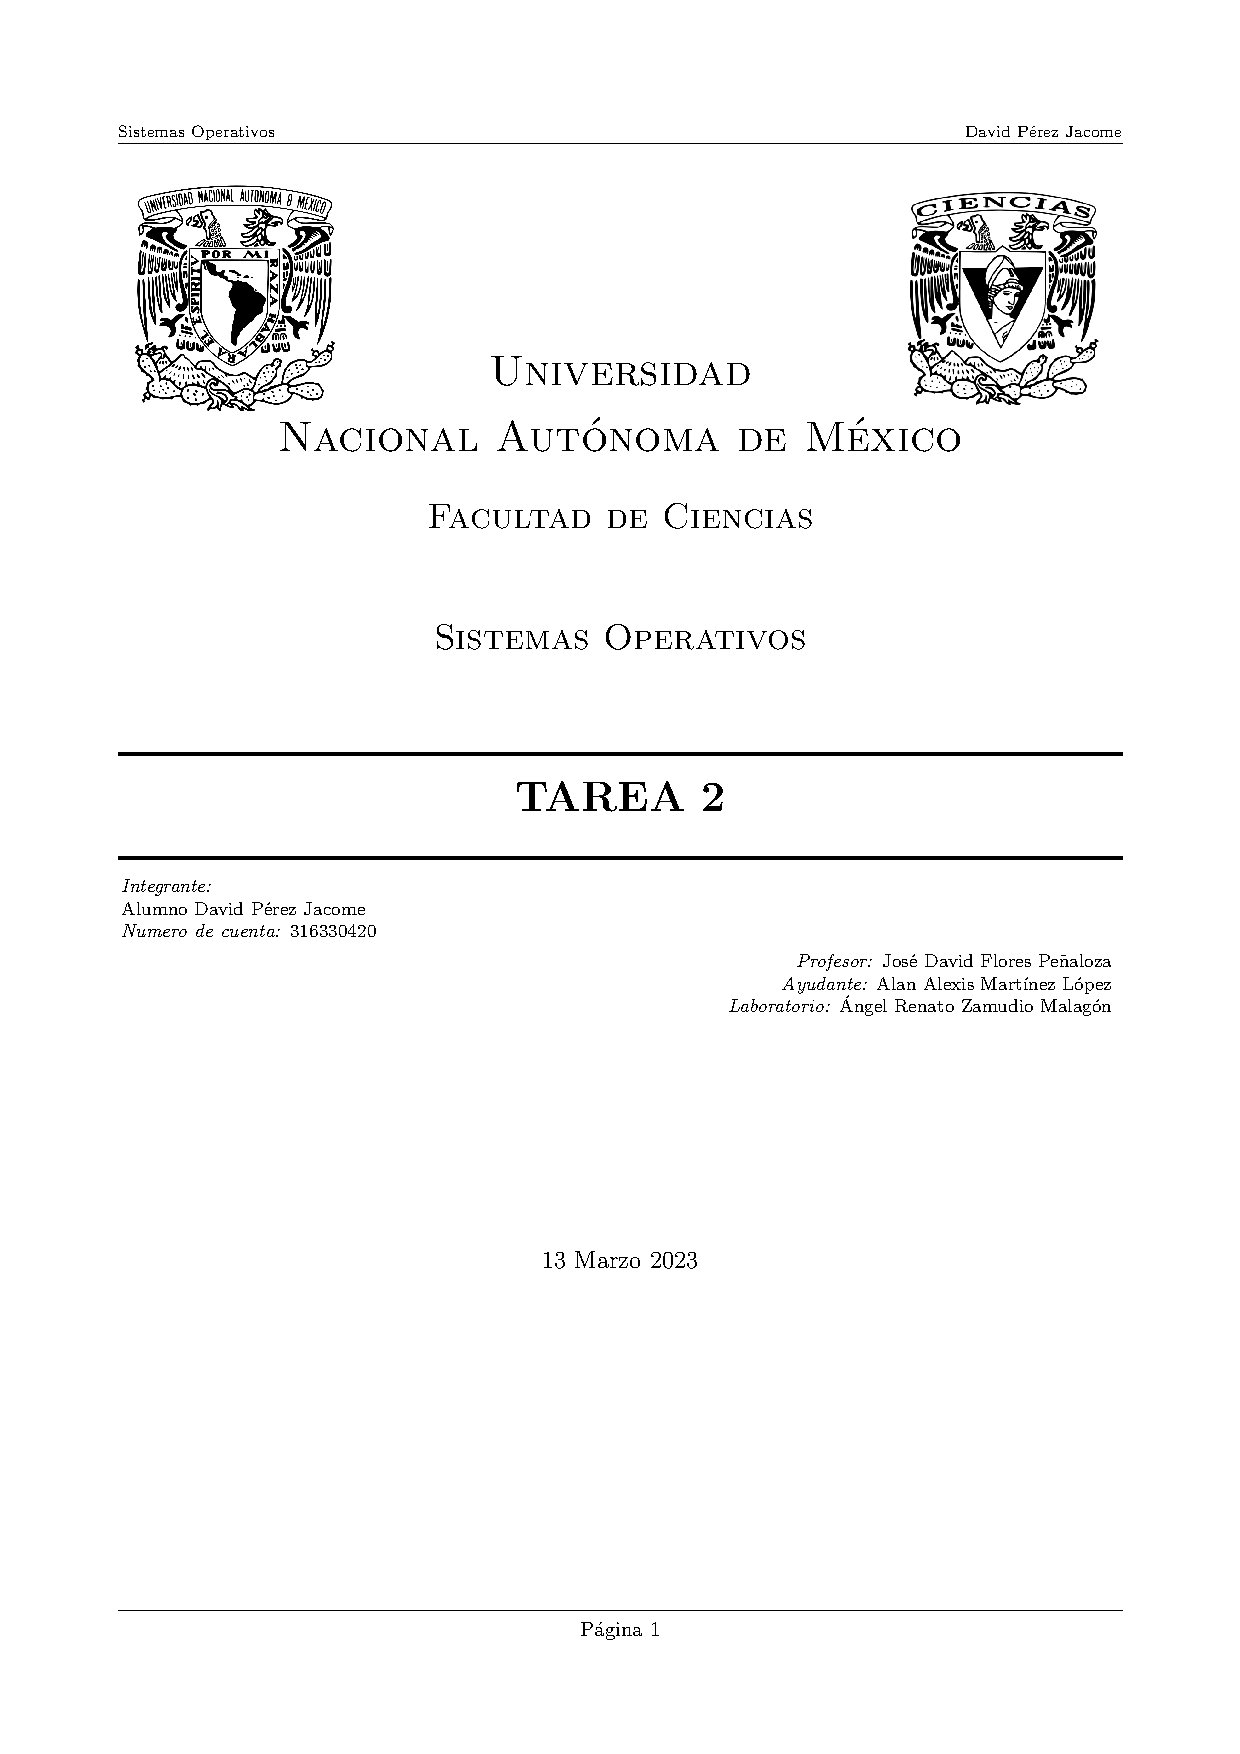
\includepdf{Portada.pdf}
{\color{blue} \section*{Tarea 2.}}

{\color{blue} \subsection*{Instrucciones.}}
\vspace{0.5em} 

Lee con atención las preguntas y contesta lo correspondiente. La tarea se entregará por vía classroom
en un archivo pdf que debe tener el nombre completo y número de tarea, ya sea en una portada o en el encabezado.
\textbf{La tarea se entregará de manera individual.}\\

{\color{blue} \subsection*{Ejercicios}}
\vspace{0.5em}

\begin{enumerate}
    \item ¿Qué es un proceso?
    \vspace{2mm}

    \textbf{Es el cambio en el estado de la memoria por acción del procesador. Es en terminos generales la unidad de trabajo del sistema operativo(calendarizable).}

    \item ¿Cuál es la diferencia entre un programa y un proceso?
    \vspace{2mm}

    \textbf{En que el proceso es una instancia de un programa en ejecución, mientras que un programa es un conjunto de instruciones y datos que describen los pasos de una tarea, o sea el ejecutable completo.}
    \item ¿Qué recursos son necesarios para el correcto funcionamiento de un proceso?
    \vspace{2mm}

    \textbf{Son 3 los recursos que son necesarios:
    \begin{enumerate}
        \item El uso del procesador o CPU.
        \item El espacio de la memoria principal.
        \item Gestión de los dispositivos de E/S.
    \end{enumerate}
    Podriamos agregar tambien Sockets y PID}
    \item ¿El procesador con que tipo de memoria puede trabajar exclusivamente?
    \vspace{2mm}

    \textbf{El procesador a la unica memoria con la que tiene un acceso exclusivo es la memoria RAM (Random Access Memory), aunque también podemos decir que tiene un acceso a la llamada 
    memoria caché, la cual si algo no esta en la cache entonces ya o busca en RAM.}

    \item Las llamadas a sistemas generalmente se hacen a través de una API ¿Por qué no hacemos llamadas al sistema invocándolas directamente?
    \vspace{2mm}

    \textbf{Para empezar si se trata de una llamada a sistema, se emplean interrupciones de la API del Kernel de Linux. Y esto no lo podemos hacer directamente porque normalmente estamos en 
    modo usuario y estos recursos estan en modo privilegiado o supervisor, por ello debemos usar n conjunto de métodos o funciones que el programa puede emplear para acceder a dichos recursos.}

    \item ¿Qué es una maquina virtual?
    \vspace{2mm}

    \textbf{Una máquina virtual (VM) es un ordenador que se ejecuta completamente en software en lugar de hardware físico. Las máquinas virtuales utilizan software en un ordenador físico (host)
    para replicar o emular la funcionalidad de un ordenador o sistema operativo diferente. En esencia, una máquina virtual es un ordenador simulado dentro de un ordenador real.}
    \item Teniendo en cuenta que es una maquina virtual. ¿Qué es un sistema operativo anfitrión y qué es un sistema operativo húesped?  
    \vspace{2mm}

    \textbf{\begin{enumerate}
        \item {\color{red}Host o Anfitrión}: Es el equipo real (un ordenador) sobre el que se ejecuta todo el sistema de virtualización. Este es mi anfitrión o host, que contendrá las máquinas virtuales.
        \item {\color{red}Huesped}: lo que se virtualiza (simula) sobre el anfitrión. Podemos crear diferentes máquinas virtuales (ordenadores simulados) que no existen realmente pero que funcionan dentro del ordenador anfitrión.
    \end{enumerate}}
    \item La maquina virtual de java ¿Es en realidad una maquina virtual? ¿De no ser así que es en realidad?
    \vspace{2mm}

    \textbf{Es un tipo de maquina virtual, se le llama {\color{red}Maquina virtual de proceso}, son máquinas virtuales permiten que ciertas herramientas se ejecuten como si fueran nativas o la funcionalidad estuviera incorporada.
    crean un entorno de programa independiente de la plataforma al ocultar la información sobre el hardware y el sistema operativo del host. }
    \item ¿Cuáles son los 3 estados que puede tener un proceso? Descríbelos
    \vspace{2mm}

    \textbf{Los procesos pueden tener 3 estados:\\
    \begin{enumerate}
        \item {\color{red}Ejecución o Activo:} Proceso que esta haciendo uso del procesador.
        \item {\color{red}Bloqueado:} No se puede ejecutar hasta que algún evento externo sea llevado a cabo.
        \item {\color{red}Preparado:} el proceso no está ejecutándose, pero es candidato a pasar a estado activo.
    \end{enumerate}} 
    \item ¿Qué es un proceso actual?
    \vspace{2mm}
    
    \textbf{Es un proceso que esta siendo ejecutado, se usa TOP para ver las estadisticas de estos procesos.}

\end{enumerate}

\end{document}